% article example for classicthesis.sty
\documentclass[10pt,a4paper]{article} % KOMA-Script article scrartcl
\usepackage{import}
\usepackage{xifthen}
\usepackage{pdfpages}
\usepackage{transparent}
\newcommand{\incfig}[1]{%
    \def\svgwidth{\columnwidth}
    \import{./figures/}{#1.pdf_tex}
}
\usepackage{lipsum}     %lorem ipsum text
\usepackage{titlesec}   %Section settings
\usepackage{titling}    %Title settings
\usepackage[margin=10em]{geometry}  %Adjusting margins
\usepackage{setspace}
\usepackage{listings}
\usepackage{amsmath}    %Display equations options
\usepackage{amssymb}    %More symbols
\usepackage{xcolor}     %Color settings
\usepackage{pagecolor}
\usepackage{mdframed}
\usepackage[spanish]{babel}
\usepackage[utf8]{inputenc}
\usepackage{longtable}
\usepackage{multicol}
\usepackage{graphicx}
\graphicspath{ {./Images/} }
\setlength{\columnsep}{1cm}

% ====| color de la pagina y del fondo |==== %
\pagecolor{white}
\color{black}



\begin{document}
    %========================{TITLE}====================%
    \title{{  Segundo Taller de Teoría de Grafos  }}
    \author{{Rodrigo Castillo}}
    \date{\today}

    \maketitle


     % ====| Loguito |==== %
    
\includegraphics[width=0.1\linewidth]{negro_cara.png}
    %=======================NOTES GOES HERE===================%
    \section{Considere el grafo G:}
        \begin{figure}[ht]
            \centering
            \incfig{grafog}
            \caption{grafo G}
            \label{fig:grafog}
        \end{figure}


        \begin{enumerate}
            \item {seleccione una arista   $ e \in E(G)  $ y dibuje $ G -e  $ y $ G
            \cdot e  $}
        \item {calcule $ r(G-e)  $  y $ r(G \cdot e)  $ }
        \item {Escriba la matriz $Q$ asociada al grafo $G$   }
        \item {Verifique $r(G)$ ,  $r(G-e) + r(G \cdot e)$ calculando $r(G)$
            por medio de la matrix $Q$ }.
        \end{enumerate}
        % ====| SOLUCION ACÁ :  |==== %



        % ====| HASTA ACA VA EL PUNTO 1 |==== %

    \newpage
    \section{Considere el digrafo D}
        % ====| digrafo G del punto 2 |==== %
        \begin{figure}[ht]
            \centering
            \incfig{digrafod}
            \caption{digrafo D}
            \label{fig:digrafod}
        \end{figure}

        \begin{enumerate}
            \item {calcule el numero de arboles de la salida de expansion de D con raíz en $u_1$ }
            \item {Calcule el número de árboles de entrada de expansión de D con raíz en $u_4$ .}
        \end{enumerate}
        % ====| SOLUCION PUNTO 2 ACÁ: |==== %




        % ====| HASTA ACA VA EL PUNTO 2 |==== %


    \newpage
    \section{Considere el grafo H}

        \begin{figure}[h!]
            \centering
            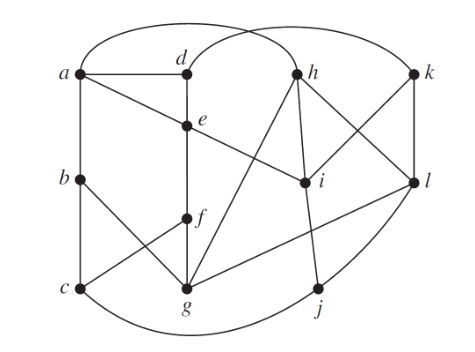
\includegraphics[width=0.5\linewidth]{grafoH.png}
            \caption{Grafo H}
            \label{grafoh}
        \end{figure}

        \begin{enumerate}
            \item {obtenga el arbol de expansión de $H$ con raíz en $g$ usando
                busqueda a profundidad.}
            \item {obtenga un árbol de expansión de $H$ con raíz en $g$ usando
                búsqueda a lo ancho}
            \item {calcule el numero de árboles de expansión de $H$ . (requiere
                programar)}
        \end{enumerate}

        % ====| SOLUCION PUNTO 3 ACA |==== %


        % ====| HASTA ACA VA EL PUNTO 3 |==== %

    \newpage
    \section{Calcule la longitud, el camino y los pasos para determinar un
    camino de longitud mínima entre $c $ y $f$ usando el algoritmo de
    \textbf{Dijkstra} en el siguiente grafo}
        \begin{figure}[h!]
            \centering
            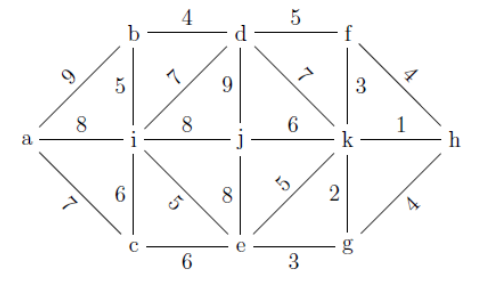
\includegraphics[width=0.5\linewidth]{grafoD.png}
            \caption{Grafo al cuál hacerle dijsktra}
            \label{bre}
        \end{figure}
        % ====| SOLUCION PUNTO 4 ACA |==== %






        % ====| Hasta acá va el punto 4 |==== %



    \newpage
    \section{Considere la siguiente tabla de frecuencias }
        \begin{figure}[h!]
            \centering
            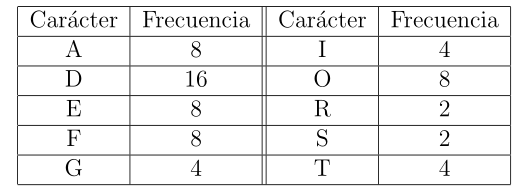
\includegraphics[width=0.5\linewidth]{frec.png}
            \caption{tabla de frecuencias}
            \label{frecuecias}
        \end{figure}

        \begin{enumerate}
            \item {Construya  un código Huffman y codifique el string
                \textbf{TEORIADEGRAFOS} }
            \item {verifique si la entropía es igual a la longitud esperada}
        \end{enumerate}
        % ====| Solución Punto 5 acá |==== %






        % ====| Hasta acá va el punto 5 |==== %

    \newpage
    \section{Escriba los recorridos pre orden , in orden y post orden de el siguiente arbol:}
        \begin{figure}[h!]
            \centering
            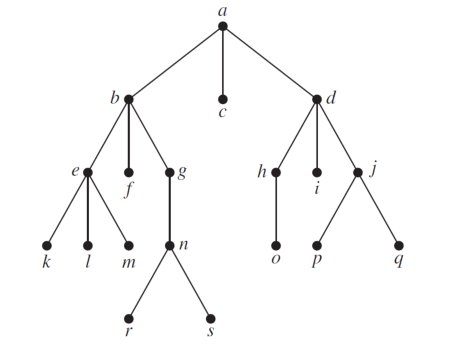
\includegraphics[width=0.5\linewidth]{arbol.png}
            \caption{Arbol}
            \label{arbol}
        \end{figure}

        % ====| Solución del punto 6 acá |==== %










        % ====| Hasta acá va el punto 6 y el taller |==== %























    %=======================NOTES ENDS HERE===================%

    % bib stuff
    \nocite{*}
    \addtocontents{toc}{{}}
    \addcontentsline{toc}{section}{\refname}
    \bibliographystyle{plain}
    \bibliography{../Bibliography}
\end{document}
